%%% BEGIN CHAPTER 3 Design of fast folding potassium channel mutant %%%

%% Paper title page %%
\chapter{Biochemical preparation of KcsA monomers and Design of fast folding KcsA mutant}
\section{Introduction}
Bacterial potassium channel, KcsA, is an extremely stable tetramer. \citep{valiyaveetil2002semi, barrera2005, barrera2008, heginbotham1997, valiyaveetil2002lipids}	Conventional denaturing reagents such as urea and guanadine do not unfold KcsA. \citep{valiyaveetil2002lipids} Sodium dodecyl sulfate (SDS) detergent is a harsh denaturing reagent for most soluble and membrane proteins; however, even SDS alone does not unfold KcsA. Only with SDS and boiling of the protein sample at 90 $^{\circ}$C for more than 10 minutes can disrupt the KcsA tetramer. So, the question is, how do we get stable monomers for biophysical studies?

In the first part of Chapter 3, a protocol for preparing KcsA monomer is presented, which are adopted from \citep{shenkarev2013} and \citep{devaraneni2011}. WT KcsA monomers were inserted into lipid nanodiscs as well as lipid bicelles for NMR studies. Through NMR and simulations, we find that the WT KcsA monomer is highly dynamic and exists in a structurally diverse ensemble of states. To stabilize the native-like state in monomers, we engineer a disulfide bond at the end of the two TM helices. This disulfide-bonded (CC) KcsA mutant monomer displays a much more native-like structure.

\section{Methods}
\subsection{KcsA expression and purification}
\subsubsection{Expression}
For KcsA expression with no isotope labeling, the protocol was adopted from \citep{tilegenova2016}. XL10-GOLD \textit{E. coli} competent cells were transformed with pQE70 KcsA WT with C-terminal 6xHis-tag using the heat shock method and grown overnight at 37 $^{\circ}$C with 1\% glucose and ampicillin (200 $\mu$g/mL). This overnight culture was used to inoculate LB media supplemented with 0.5\% glycerol, 0.2\% glucose and ampicillin (200 $\mu$g/mL) at a final concentration of 1\% v/v. Once this culture reached OD$_{600}$ $\sim$ 0.6 and they were cooled down to 29 $^{\circ}$C for 1 hour. Then, protein expression was induced with 0.1 mM Isopropyl $\beta$-D-1-thiogalactopyranoside (IPTG), 10mM BaCl2 (K+ channel blocker) and 0.2 $\mu$g/mL ampicillin. Cells were incubated overnight at 29 $^{\circ}$C and harvested after 14 -- 18 hours of growth by centrifuging at 9,000 RCF for 15 minutes at 4 $^{\circ}$C. The pellet was stored in -70 $^{\circ}$C until purification.

For expressions with isotope labeling for NMR studies, the protocol was adopted from \citep{bhate2013}. JM83 \textit{E. coli} competent cells were transformed with pASK90 KcsA with N-terminal 6xHis-tag and grown overnight at 37 $^{\circ}$C with ampicillin (200 $\mu$g/mL). The overnight culture was used to inoculate a 100 mL of LB media with ampicillin (200 $\mu$g/mL) and was grown until OD$_{600}$ reached 0.5. This culture was then used to inoculate 4 L of LB media by adding 1\% of the total volume. The 4 L of LB were grown until OD$_{600}$ reached $\sim$ 0.9 and were spun down at 4,000 RCF for 10 minutes at 4 $^{\circ}$C. The biomass was quadrupled by combining cell pellets from 4 L of LB media into 1 L of M9 media. The pellet was resuspended with 40 mL of M9 media and returned to 1 L of M9 media. The cells were allowed to acclimate for an hour at 37 $^{\circ}$C and then were induced with 0.2mg/L anhydrotetracycline (aTC). Pellets were harvested 12 –- 14 hours later by spinning down at 9,000 RCF for 15 minutes at 4 $^{\circ}$C. After the pellet was spun down, the pellet was frozen in -70 $^{\circ}$C until purification. 

For the M9 media, the ingredients are shown in Tables \ref{table:ch3_t1}, \ref{table:ch3_t2} and \ref{table:ch3_t3}. For vitamin stock solution, one multi-purpose vitamin purchased from CVS is crushed using mortar and pestle. The crushed vitamin is then solubilized in deionized water in 20 mL volume. This solution is then sterile filtered and stored in -20 $^{\circ}$C. When making the M9 media, Na$_{2}$HPO$_{4}$, KH$_{2}$PO$_{4}$, NaCl are first mixed together and autoclaved. Rest of the ingredients are added after autoclave.
\begin{table}[h]
\centering
	\caption{Ingredients for 1L of M9 media}
	\begin{tabular}{cc}
	\hline
	Ingredients & Amount \\
	\hline
	Na$_{2}$HPO$_{4}$     & 12.8 g  \\
	KH$_{2}$PO${4}$      & 3 g \\
	NaCl & 0.5 g \\
	Solution C & 20 mL \\
	MgSO$_{4}$ & 0.1 g \\
	CaCl$_{2}$ & 0.01 g \\
	FeCl$_{2}$ & 0.01 g \\
	Thiamine & 0.01 g \\
	Glucose & 3 g \\
	NH$_{4}$Cl & 1 g \\
	L-Proline & 1 g \\
	Vitamin Stock & 2 mL \\
	Ampicillin & 0.2 g \\
	\hline
	\end{tabular}
	\label{table:ch3_t1}
	\end{table}

\begin{table}[!htb]
%\centering
    \begin{minipage}{.5\linewidth}
	  \caption{1 L of Solution C \\ adjust pH to 6.7}
      \centering
		\begin{tabular}{cc}
		\hline
		Ingredients & Amount \\
		\hline
		KOH & 7.3 g  \\
		Metal 44 & 50 mL \\
		Nitrilotriacetic acid & 10 g \\
		MgCl$_{2}$ 6H$_{2}$O & 24 g \\
		CaCl$_{2}$ 2H$_{2}$O & 3.335 g \\
		\hline
		\end{tabular}
		\label{table:ch3_t2}
    \end{minipage}
    \begin{minipage}{.5\linewidth}
		\caption{100 mL of Metal 44 Solution, \\store in dark glass bottle at 4 $^{\circ}$C}
		\centering
		  \begin{tabular}{cc}
	  	  \hline
		  Ingredients & Amount \\
 	      \hline
	      K$_{2}$EDTA 2H$_{2}$O  & 0.327 g  \\
          ZnCl$_{2}$ & 0.522 g \\
		  FeCl$_{2}$ 4H$_{2}$O & 0.502 g \\
		  MnCl$_{2}$ 4H$_{2}$O & 0.18 g \\	
		  (NH$_{4}$)$_{6}$Mo$_{7}$O$_{24}$ 6H$_{2}$O & 0.0185 g \\
		  CuCl$_{2}$ 2H$_{2}$O & 0.0156 g \\
		  Co(NO$_{3}$)$_{2}$ 6H$_{2}$O & 0.0248 g \\
		  Boric Acid & 0.0114 g \\
		  \hline
		  \end{tabular}
		  \label{table:ch3_t3}
    \end{minipage} 
\end{table}

\subsubsection{Purification}
For purification, the frozen pellets were resuspended in buffer A (50 mM HEPES, 200 mM KCl, pH 7.0) with 1 mM phenylmethylsulfonyl fluoride (PMSF), 3 mg of DNAse A (Goldbio) per liter of culture, and 0.4 mM MgSO$_{4}$. The cells were lysed through 3x passage through french press, and the lysed cells were spun down at 158,000 RCF for 30 minutes at 4 $^{\circ}$C. The pellet was resuspended in buffer A with 10 mM n-dodecyl $\beta$-D-maltoside (DDM) and 1 mM PMSF. The mixture was rotated at room temperature for 1 hour to extract and solubilize KcsA in DDM. Then, the mixture was spun down at 185,000 RCF for 1 hour at 4 $^{\circ}$C. Supernatant was incubated with Talon Metal Affinity Co2+ resins and rotated at room temperature for 1 hour. The resins were then collected by gravity and the flow through was discarded. The columns were washed with 15 bed volumes of Buffer A + 1 mM DDM + 10 mM imidazole and the proteins were eluted with Buffer A + 1 mM DDM + 500 mM imidazole.

For full-length KcsA constructs, protein in elution solution was further purified by size-exclusion chromatography on Superdex 200 Increase column that was pre-equilibrated with Buffer containing 50 mM NaPi, 100 mM NaCl, 1 mM DDM, pH 7. For KcsA $\Delta$125 constructs, full length KcsA constructs were first trypsinized with $\alpha$-chymotrypsin (Sigma Aldrich) at 4 $^{\circ}$C overnight with 1:50 (chymotrypsin:KcsA) ratio. Then, the digested KcsA was further purified through size-exclusion chromatography (SEC) with Superdex 200 Increase column. 

\subsection{Design and production of fast folding KcsA mutant}
Based on previous simulations of WT Kv1.2 and KcsA monomers as well as NMR results shown in \textit{Results} section of this chapter, potassium channel pore domain monomers seemed to be highly dynamic and structurally heterogeneous. In order to limit the dynamical nature of WT KcsA monomer, we introduce a disulfide bridge at the end of the two TM helices to limit its dynamical nature. The residues chosen for mutations are A29 and A109, and both were mutated using the QuickChange protocol. For expression and purification, the protocol is identical to expression and purification of WT KcsA discussed in the previous section.

\subsection{KcsA monomer preparation}
\begin{figure}[!ht]
\begin{center}
	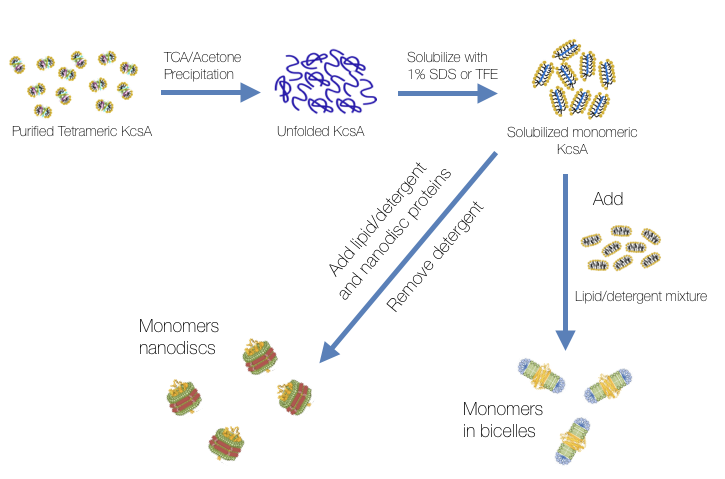
\includegraphics[width=\textwidth]{figures/chapter3/monomer_prep.png}
\end{center}
	\caption{\textbf{Protocol for preparing monomeric KcsA in nanodisc or bicelle}}
	\label{fig:ch3_f1}
\end{figure}

For preparing monomer samples, we follow the protocol highlighted in Figure \ref{fig:ch3_f1}. Purified tetrameric KcsA after SEC step are all pooled together, and they are precipitated by adding 15\% v/v tricholoroacetic acid (TCA) to the samples. The precipitated samples were frozen at -70 $^{\circ}$C for 30 minutes. Then, the frozen samples were spun down at 16,200 RCF for 30 minutes at 4 $^{\circ}$C. Supernatant was removed, and washed with chilled (-20 $^{\circ}$C) acetone. Precipitates were resuspended, vortexed for 30 seconds, and incubated at -20 $^{\circ}$C for 30 minutes until spin down at 16,200 RCF for 15 minutes at 4 $^{\circ}$C. This acetone wash step was repeated 3 times. The final precipitate was dried under air until all acetone evaporated, and the precipitate was stored in -80 $^{\circ}$C until usage. For solubilizing the precipitated monomers, either 1\% SDS or 100\% TFE is used.

\subsubsection{KcsA monomer in nanodisc}
The protocol for kinetically trapping KcsA monomer in nanodisc was adopted from \citep{hagn2013} and \citep{ritchie2009}. First, 0.5\% SDS-solubilized KcsA monomers is mixed with 1,2-dimyristoyl-sn-glycero-3-phosphoglycerol (DMPG) and sodium cholate. Typically, DMPG is mixed with cholate at ratio of 1:2. Optimal protein to lipid ratio was determined empirically at 1:5 by checking the monodispersity of size-exlusion chromatography (SEC) elution profile. After an hour of mixing at room temperature, 1 g of Biobead SM-2 is added per mL of nanodisc mixture. Then, the mixtures with Biobeads is further mixed for overnight at room temperature. Biobeads were removed by centrifugation and nanodiscs were further purified by SEC using Superdex 200 Increase column. 

\subsubsection{KcsA monomer in bicelle}
KcsA monomers in bicelles were prepared in q=0.3 DMPC:DHPC bicelles using following procedure. Bicelle mixture was first prepared by adding 1:3 molar ratio of DMPC or POPC to DHPC (both solubilized in chloroform) at final lipid concentration of 10\% w/v in the NMR sample. Chloroform was evaporated under stream of nitrogen and further removed under vacuum for 3 –- 4 hours. This procedure resulted in a thin lipid film, which was resolubilized in 2,2,2-trifluoroethanol (TFE). WT KcsA $\Delta$125 precipitate is solubilized in TFE and mixed into the lipid TFE mixture. TFE was evaporated under a stream of nitrogen until a thin film formed around the glass tube and was further evaporated by placing the tube under vacuum overnight. Then, the thin lipid film was rehydrated with buffer of choice and vortexed for 30 seconds. Typically for NMR, the buffer contained 20 mM NaPi, 50 mM NaCl, 0.03\% NaN$_{3}$, and pH6.5. 

\subsection{Nuclear magnetic resonance (NMR) measurements of KcsA}
NMR spectra were acquired on Bruker AVANCE IIIHD 600 MHz NMR spectrometer equipped with a room temperature TXI probe. [$^{1}$H, $^{15}$N]-TROSY HSQC experiments were run at T=323 K. To obtain rotational correlation times, $\tau_{c}$, [15N, 1H]-TRACT experiments were performed. \citep{lee2006, cavanagh2007, cho1999, nesg2011, pond2012} 

\subsection{KcsA CC simulations and MSM analysis}
The starting structure for KcsA monomer simulations was taken from the tetrameric KcsA X-ray crystal structure (PDB ID: 1R3J). Mutations were made at A29C and A109C for the disulfide mutant simulations, and disulfide bond was created using CHARMM-GUI’s PDBReader module. All systems were prepared by using CHARMM-GUI’s Membrane Builder module (www.charmm-gui.org)64-68. Each system contained 70 1,2-dimyristoyl-sn-glycero-3-phosphatidylcholine (DMPC) molecules per leaflet totaling up to 140 DMPC molecules to match the NMR sample conditions. All systems were hydrated by creating a water box 17.5 Å above and below the protein’s maximum and minimum Z-positions. In addition, the system was neutralized with 150 mM KCl. The system comprised a total of approximately 45,000 atoms. 5 independent simulations of KcsA WT monomer and 5 simulations of KcsA CC mutant monomer were carried out at T = 353 K to enhance sampling. All simulations were run with the parameters described in Methods section with AMBER16 GPU, and each simulation was run up to 6 $\mu$s. In total 30 $\mu$s of KcsA WT simulations and 30 $\mu$s of KcsA CC simulations were accumulated.

For MSM analysis, all KcsA simulations were first projected onto the TIC space created by Kv1.2 simulations. KcsA monomer has 103 residues in total whereas Kv1.2 pore domain has 99 residues. In order to project KcsA monomer simulations, C$\alpha$ atoms were aligned to Kv1.2 structure. The final corresponding residues in KcsA were from residues 24 to 122, which were used for TICA projection. After projecting KcsA simulations onto the same TIC space as Kv1.2, all simulations were combined in order to create the same number of microstates using K-Center clustering algorithm. After the same microstates were created, Markov state model constructions were done as described in SI Methods. However, MSM was constructed separately for Kv1.2, KcsA WT and KcsA CC using the same set of microstates.

\section{Results and Discussion}
\subsection{WT KcsA monomers are structurally diverse}

Expression and purification of KcsA tetramers is straightforward. Many labs can reliably produce large amounts of KcsA for biophysical studies. \citep{chill2007, valiyaveetil2002semi, barrera2005, tilegenova2016, bhate2013, takeuchi2007, cortes1997} KcsA $\Delta$125 constructs are prepared by incubating KcsA full-length (FL) constructs with $\alpha$-chymotrypsin at 1:50 ratio overnight at 4 $^{\circ}$C. Then, the KcsA $\Delta$125 are purified from chymotrypsin by size-exclusion chromatography (SEC) with Superdex 200 Increase column as shown in Figure \ref{fig:ch3_f2}B.

\begin{figure}[!ht]
\begin{center}
	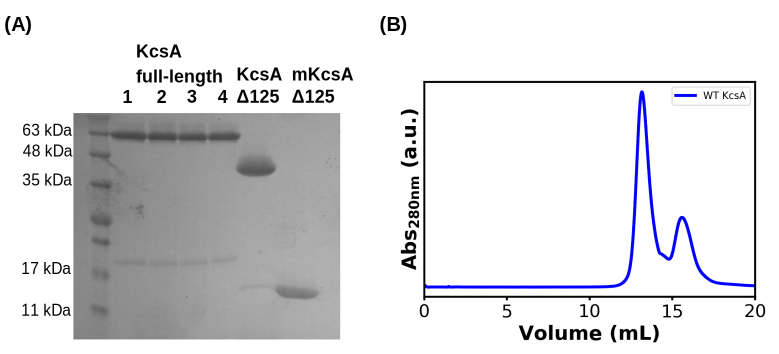
\includegraphics[width=\textwidth]{figures/chapter3/wtkcsa_gel_sec.pdf}
\end{center}
	\caption{\textbf{Purification of KcsA} \textbf{(A)} SDS-PAGE gel with KcsA full-length (FL), KcsA $\Delta$125, monomeric KcsA (mKcsA) $\Delta$125. \textbf{(B)} Elution profile of WT KcsA $\Delta$ tetramer with chymotrypsin. KcsA $\Delta$125 elutes around 13 mL and chymotrypsin elutes near 16 mL.}
	\label{fig:ch3_f2}
\end{figure}

KcsA monomers are prepared by trichloroacetic acid (TCA)/Acetone precipitation protocol as discussed in \textit{Methods} section. The precipitate monomers can be solubilized in 0.5\% SDS and is shown to run as 13 kDa on SDS-PAGE (\textbf{Fig. \ref{fig:ch3_f2}}). The monomers were then transferred to nanodisc or bicelle for NMR studies.

\begin{figure}[!ht]
\begin{center}
	\includegraphics[width=\textwidth]{figures/chapter3/wt_nmr.pdf}
\end{center}
	\caption{\textbf{[$^{15}$N-$^{1}$H]-TROSY-HSQC spectra of KcsA WT.}  \textbf{(A)} HSQC of KcsA $\Delta$125 solubilized in MSP1D1 $\Delta$H5 nanodisc is shown. \textbf{(B)} HSQC of KcsA $\Delta$125 solubilized in q=0.3 DMPC:DHPC bicelle is shown.}
	\label{fig:ch3_f3}
\end{figure}

NMR spectra of WT KcsA in either MSP1D1 $\Delta$H5 or q=0.3 DMPC:DHPC bicelle do not show well-resolved peaks in general. In fact, for WT KcsA solubilized in bicelle easily forms soluble aggregates in the NMR sample conditions. In Chapter 2, we found that Kv1.2 and KcsA monomers seem to be structurally diverse through MD simulations and Markov state model analysis. Given our NMR spectra and the computational modelling results, we suspect that the WT KcsA monomers are structurally heterogeneous in lipid bilayers. 

\subsection{Designing more native-like KcsA mutant}

With the KcsA mutant

\begin{figure}[!ht]
\begin{center}
	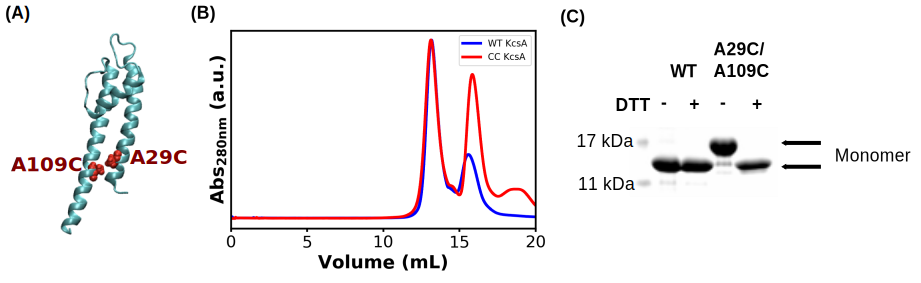
\includegraphics[width=\textwidth]{figures/chapter3/cc_sec_gel.pdf}
\end{center}
	\caption{\textbf{[$^{15}$N-$^{1}$H]-TROSY-HSQC spectra of KcsA WT.}  \textbf{(A)} HSQC of KcsA $\Delta$125 solubilized in MSP1D1 $\Delta$H5 nanodisc is shown. \textbf{(B)} HSQC of KcsA $\Delta$125 solubilized in q=0.3 DMPC:DHPC bicelle is shown.}
	\label{fig:ch3_f4}
\end{figure}

\subsection{NMR of potassium channel monomers}

\begin{figure}[!ht]
\begin{center}
	\includegraphics[width=\textwidth]{figures/chapter3/nmr.pdf}
\end{center}
	\caption{\textbf{Simulation comparison between Kv1.2 and KcsA.} \textbf{(A)} Number of contacts between the 2 transmembrane helices are plotted as a function of simulation time. \textbf{(B)} RMSD of the overall monomer is plotted as a function of time. \textbf{(C)} Kv1.2 and KcsA simulations are projected onto the same TIC space. Markov state model is made using the same set of microstates and the correponding free energy surface is plotted}
	\label{fig:ch3_f5}
\end{figure}

\section{Conclusion}

%% REVERT FIGURE NUMBERING %%
\renewcommand\thefigure{\thechapter.\arabic{figure}} 

%%% END CHAPTER 2 Design of fast folding potassium channel mutant %%%
